%=============================================================================%
% Author: 	John Joseph Valletta
% Date: 	10/03/2017
% Title: 	Introduction to Python Workshop
%=============================================================================%

%=============================================================================%
% Preamble
%=============================================================================%
% Libraries
\documentclass[pdf]{beamer}
\usepackage[export]{adjustbox}
\usepackage{framed}
\usepackage{color}
\definecolor{dkgreen}{rgb}{0,0.6,0}
\definecolor{gray}{rgb}{0.5,0.5,0.5}
\definecolor{mauve}{rgb}{0.58,0,0.82}
\definecolor{deepblue}{rgb}{0,0,0.5}
\definecolor{deepred}{rgb}{0.6,0,0}
\definecolor{deepgreen}{rgb}{0,0.5,0}
\definecolor{lightgray}{rgb}{0.92,0.92,0.92}
\usepackage{listings} % to insert code
\usepackage{textpos} % textblock
\usepackage{hyperref}
\hypersetup{colorlinks=true, urlcolor=blue, linkcolor=black} 

% Listing set up
% bash
\lstdefinestyle{bash}{
language=bash,                     % the language of the code
basicstyle=\scriptsize\ttfamily,       % the size of the fonts that are used for the code
numbers=none,%left,                   % where to put the line-numbers
numberstyle=\tiny\color{gray},  % the style that is used for the line-numbers
stepnumber=1,                   % the step between two line-numbers. If it's 1, each line
                          % will be numbered
numbersep=5pt,                  % how far the line-numbers are from the code
backgroundcolor=\color{lightgray},  % choose the background color. You must add \usepackage{color}
showspaces=false,               % show spaces adding particular underscores
showstringspaces=false,         % underline spaces within strings
showtabs=false,                 % show tabs within strings adding particular underscores
frame=lines,%single,                   % adds a frame around the code
rulecolor=\color{black},        % if not set, the frame-color may be changed on line-breaks within not-black text (e.g. commens (green here))
tabsize=2,                      % sets default tabsize to 2 spaces
captionpos=b,                   % sets the caption-position to bottom
breaklines=true,                % sets automatic line breaking
breakatwhitespace=false,        % sets if automatic breaks should only happen at whitespace
title=\lstname,                 % show the filename of files included with \lstinputlisting;
                          % also try caption instead of title
keywordstyle=\color{blue},      % keyword style
commentstyle=\color{dkgreen},   % comment style
stringstyle=\color{mauve},      % string literal style
escapeinside={\%*}{*)},         % if you want to add a comment within your code
morekeywords={}            % if you want to add more keywords to the set
}

% Python
\lstdefinestyle{python}{
language=python,
formfeed=\newpage,
basicstyle=\scriptsize\ttfamily,
commentstyle=\color{deepgreen},%\color{gray},
numbers=left,
numberstyle=\tiny\color{gray},
stepnumber=1,
numbersep=5pt,
backgroundcolor=\color{lightgray},%\color{white},
showspaces=false,
showstringspaces=false,
showtabs=false,
frame=lines,
tabsize=4,
captionpos=b,
breaklines=true,
breakatwhitespace=false,
title=\lstname,
escapeinside={},
keywordstyle=\color{deepblue},
emphstyle=\color{deepred},
stringstyle=\color{deepgreen}
%morekeywords={models, lambda, forms}
}

% Presentation configuration
\mode<presentation>{\usetheme{Madrid}}
\definecolor{tealblue}{rgb}{0, 0.5, 0.5}
\usecolortheme[named=tealblue]{structure}
\useinnertheme{circles} % circles, rectanges, rounded, inmargin
\usefonttheme[onlymath]{serif} % makes math fonts like the usual LaTeX ones
\setbeamercovered{transparent=4} % transparent
\setbeamertemplate{caption}{\raggedright\insertcaption\par} % Remove the word "Figure" from caption %\setbeamertemplate{caption}[default]
\setbeamertemplate{navigation symbols}{} % don't put navigation tools at the bottom (alternatively \beamertemplatenavigationsymbolsempty)
\graphicspath{ {../images/} }

% Titlepage
\title[Python for scientific research]{Python for scientific research}
\subtitle{Introduction}
\author{John Joseph Valletta}
\date[June 2017]{June 2017}
\institute[]{University of Exeter, Penryn Campus, UK}
\titlegraphic{
\hfill

\includegraphics[width=\textwidth, keepaspectratio]{logo.jpg}}

%=============================================================================%
%=============================================================================%
% Start of Document
%=============================================================================%
%=============================================================================%
\begin{document}

%=============================================================================%
%=============================================================================%
\begin{frame}
\titlepage
\end{frame}

%=============================================================================%
%=============================================================================%
\begin{frame}{Acknowledgements}
\begin{itemize}\addtolength{\itemsep}{\baselineskip}
	\item The workshop is funded by Exeter's researcher-led initiative award 
	\item Thanks to \href{http://www.exeter.ac.uk/biomedicalhub/team/drjeremymetz/}{Jeremy Metz} for sharing his \href{https://metzjp.bitbucket.io/}{notes} used in the Biomedical Informatics Hub, from which I borrowed some examples 
	\item Last but not least, big thanks to Mario Recker, Thomas Holding, Warren Tennant and James Clewett for helping out putting this workshop together
\end{itemize}
\vfill

\includegraphics[width=\textwidth, keepaspectratio]{logo.jpg}

\end{frame}

%=============================================================================%
%=============================================================================%
\begin{frame}{Housekeeping}

\centering
\includegraphics<1>[width=\textwidth]{day1.pdf}
\includegraphics<2>[width=\textwidth]{day2.pdf}

\end{frame}

%=============================================================================%
%=============================================================================%
\begin{frame}{References}

\begin{itemize}\addtolength{\itemsep}{\baselineskip}
	\item \href{https://python.swaroopch.com/}{A Byte of Python}
	\item \href{http://greenteapress.com/wp/think-python/}{Think Python}
	\item \href{http://www.southampton.ac.uk/~fangohr/training/python/pdfs/Python-for-Computational-Science-and-Engineering.pdf}{Python for Computational Science and Engineering}
	\item \href{https://hplgit.github.io/primer.html/doc/pub/half/book.pdf}{A Primer on Scientific Programming with Python}
	\item \href{https://www.kevinsheppard.com/Python_for_Econometrics}{Introduction to Python for Econometrics, Statistics and Numerical Analysis}
\end{itemize}

\end{frame}

%=============================================================================%
%=============================================================================%
\begin{frame}{What is Python?}
% Monty Python figure
\centering
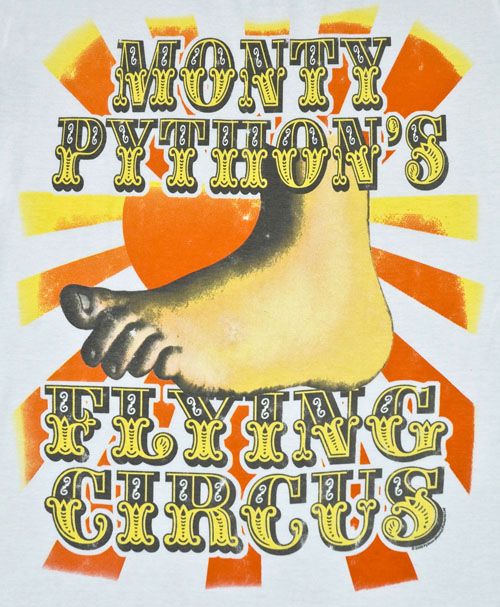
\includegraphics[width=0.35\textwidth]{monty_python.jpg}

\small
\begin{itemize}\addtolength{\itemsep}{.2\baselineskip}
	\item<2-> A scripted high-level programming language created by \href{https://en.wikipedia.org/wiki/Guido_van_Rossum}{Guido Van Rossum} and named after \href{https://en.wikipedia.org/wiki/Monty_Python's_Flying_Circus}{Monty Python's Flying Circus}
	\item<3-> Easy-to-use, versatile and with an emphasise on readability
	\item<4-> It has a minimalistic English-like syntax, relying on indentation instead of curly brackets, semicolons etc. 
\end{itemize}
\normalsize

\end{frame}

%=============================================================================%
%=============================================================================%
\begin{frame}{Why Python?}
The \href{http://www.tiobe.com/tiobe-index/}{TIOBE index} is a measure of the popularity of programming languages

% Tiobe index
\centering
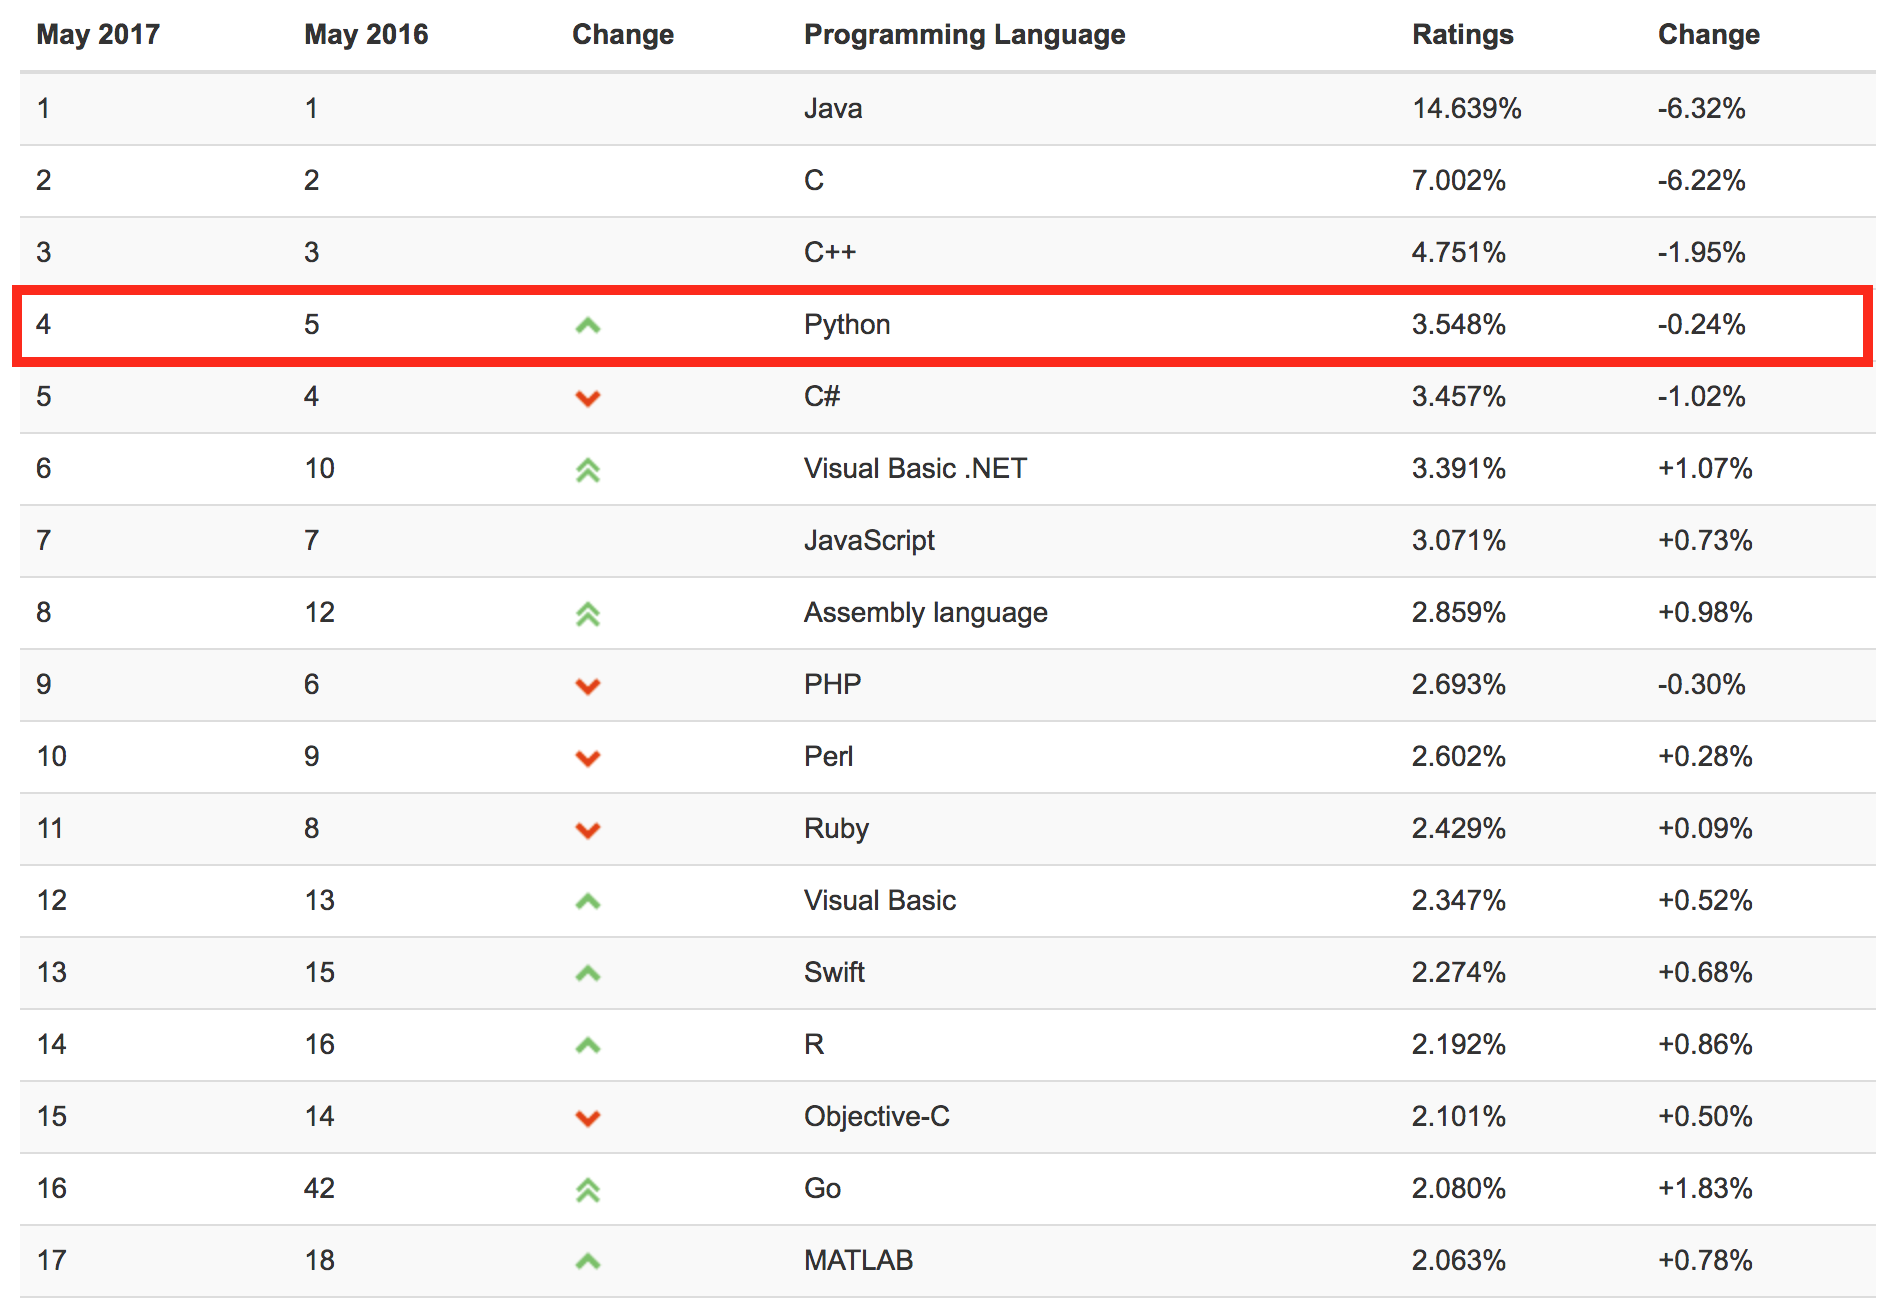
\includegraphics[width=.85\textwidth]{tiobe.png}
\end{frame}

%=============================================================================%
%=============================================================================%
\begin{frame}{Why Python?}
%. Here are some reasons for its popularity:

\begin{itemize}\addtolength{\itemsep}{0.5\baselineskip}
	\item<1-> It is free! No licence costs
	\item<2-> Runs on all platforms (Mac, Windows, Linux)
	\item<3-> Because of it's ease of programming (e.g no neeed to worry about memory allocation), Python minimises development effort
	\item<4-> A huge number of \href{https://pypi.python.org/pypi}{libraries}, written by an active \href{https://www.python.org/community/}{community}  
	\item<5-> Python can ``glue" together functions written in C/C++ and Fortran to speed things up (we can also call R and MATLAB functions)
	\item<6-> Compared to other high-level scientific languages such as MATLAB and R, Python offers a much wider range of additional functionality (e.g \href{https://www.djangoproject.com/}{web} and \href{https://wiki.python.org/moin/TkInter}{GUI} development) %hence the nickname ``the swiss army knife" of programming languages. 
\end{itemize}

\end{frame}

%=============================================================================%
%=============================================================================%
\begin{frame}{Horses for courses}

\begin{itemize}\addtolength{\itemsep}{0.5\baselineskip}
	\item<1-> Python is becoming the de facto standard for exploratory and interactive scientific research\\
	\item[]<1-> \textbf{BUT}
	\item<2-> Python is no programming silver bullet
	\item<3-> Your application will ultimately dictate the tool (and a mixture of more than one language \textbf{is} ok). For example:\\
	\begin{itemize}\addtolength{\itemsep}{0.8\baselineskip}
		\item<4-> MATLAB excels at interfacing with hardware, e.g generating \href{https://uk.mathworks.com/products/hdl-coder.html}{hardware description language (HDL) code} to configure an integrated circuit board or connecting to a \href{https://uk.mathworks.com/products/daq.html}{data acquisition card}
		\item<5-> R is great for data wrangling and visualisation, and statistical modelling
		\item<6-> \href{http://mc-stan.org/}{Stan} (a probabilistic programming language) is an excellent choice for performing full Bayesian statistical inference
	\end{itemize}
\end{itemize}

\end{frame}

%=============================================================================%
%=============================================================================%
\begin{frame}{Why do \textit{you} want to learn Python?}
% Word cloud
\centering
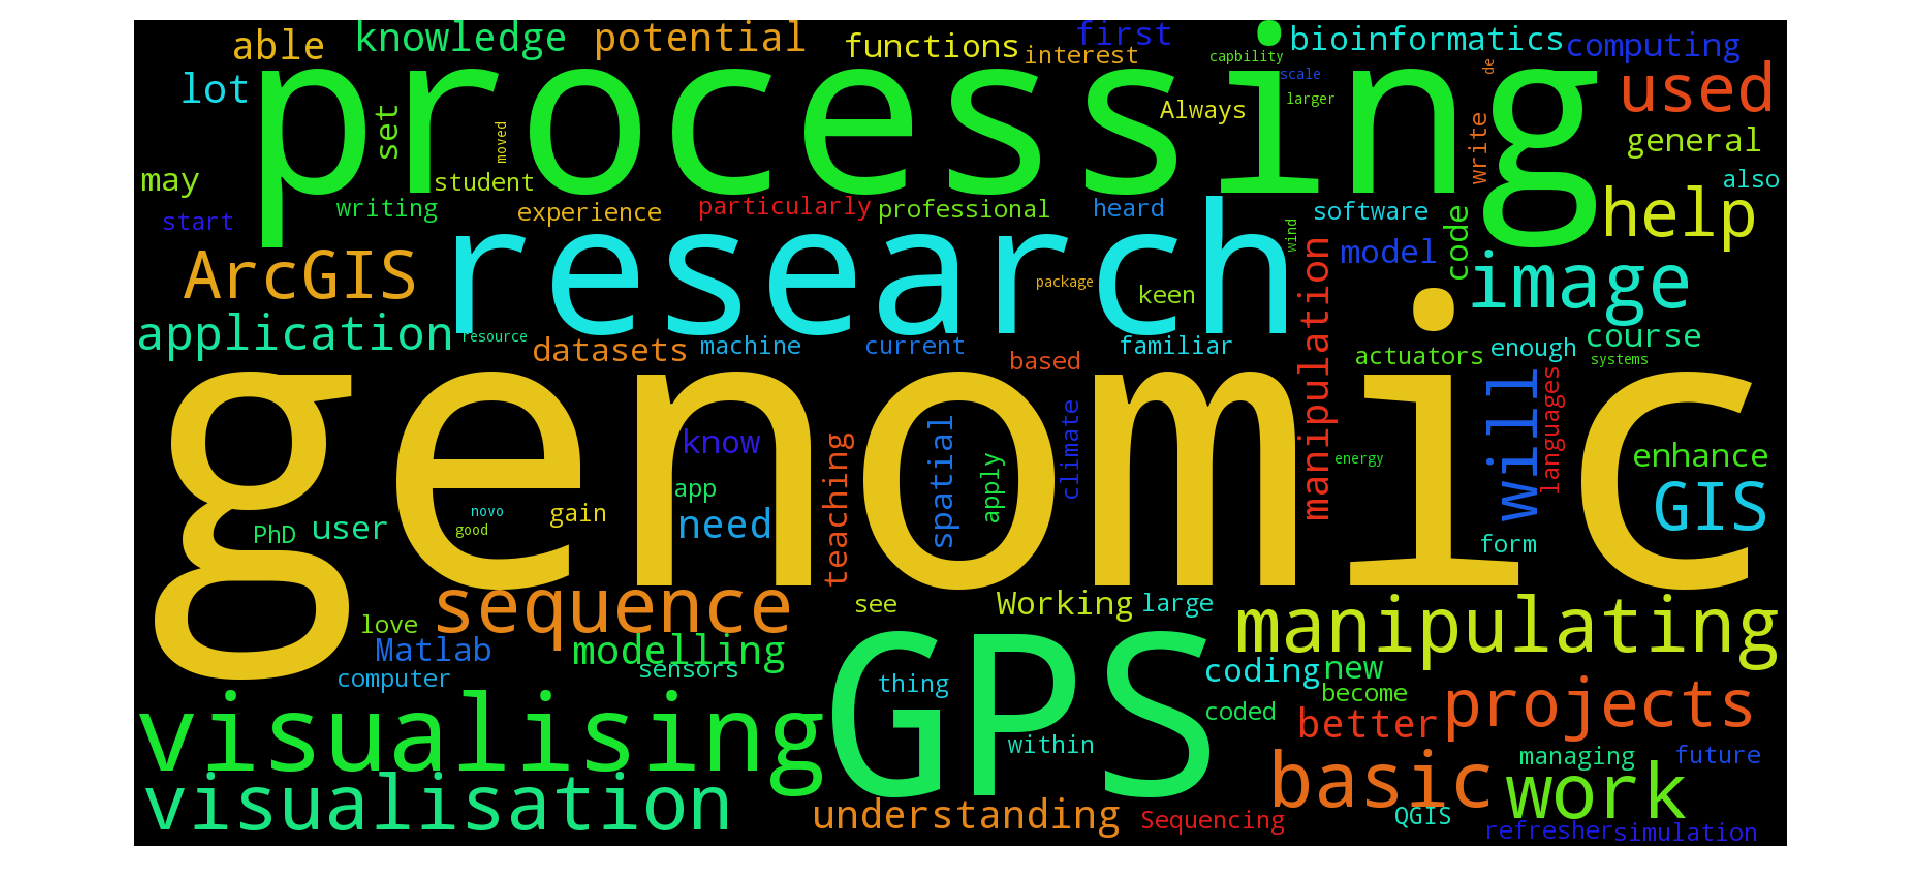
\includegraphics[width=\textwidth]{wordcloud.png}
\end{frame}

%=============================================================================%
%=============================================================================%
\begin{frame}[fragile]
\frametitle{Executing Python code: No frills Python interpreter}

\begin{itemize}\addtolength{\itemsep}{0.5\baselineskip}
	\item Type \texttt{python} in your terminal window to invoke the interpreter
	\item Any Python code you type in is executed once you press enter  
\end{itemize}

\centering
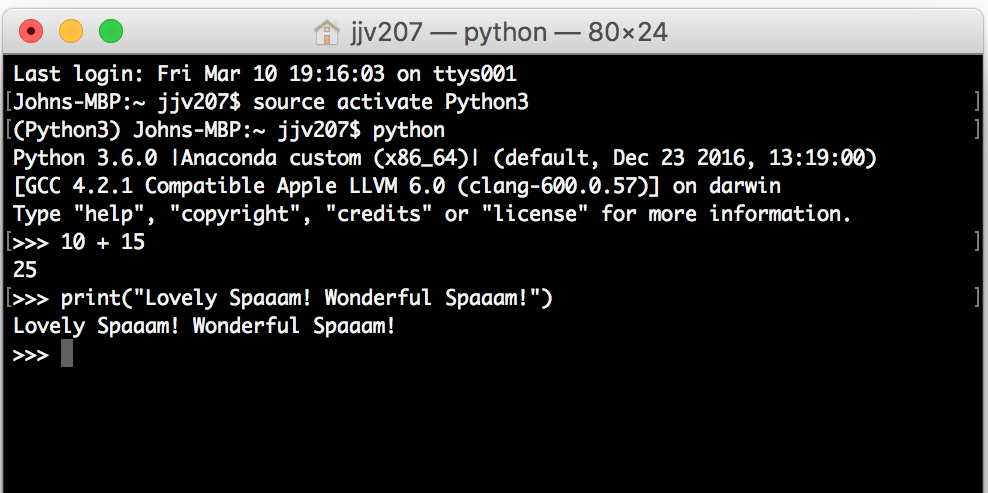
\includegraphics[width=0.75\textwidth]{python_interpreter.png}

\begin{itemize}\addtolength{\itemsep}{0.5\baselineskip}
	\item Alternatively if your code is written in a text file, e.g \texttt{my\_script.py}:
\end{itemize}

\begin{lstlisting}[style=bash]
python my_script.py
\end{lstlisting}

\end{frame}

%=============================================================================%
%=============================================================================%
\begin{frame}[fragile]
\frametitle{Executing Python code: IPython interpreter}
\begin{itemize}
	\item IPython is an interactive shell (similar to R Console), adding ``frills" to the vanilla interpreter, such as:

	\begin{itemize}
		\item syntax highlighting (making it easier to read code)
		\item tab auto-completion (minimises typeos and lists available functions)  
	\end{itemize}
	%\item The IPyton interactive shell is what powers Jupyter in the background (i.e code that I write in these notes is interpreted and executed by the IPython shell)
\end{itemize}

\begin{center}
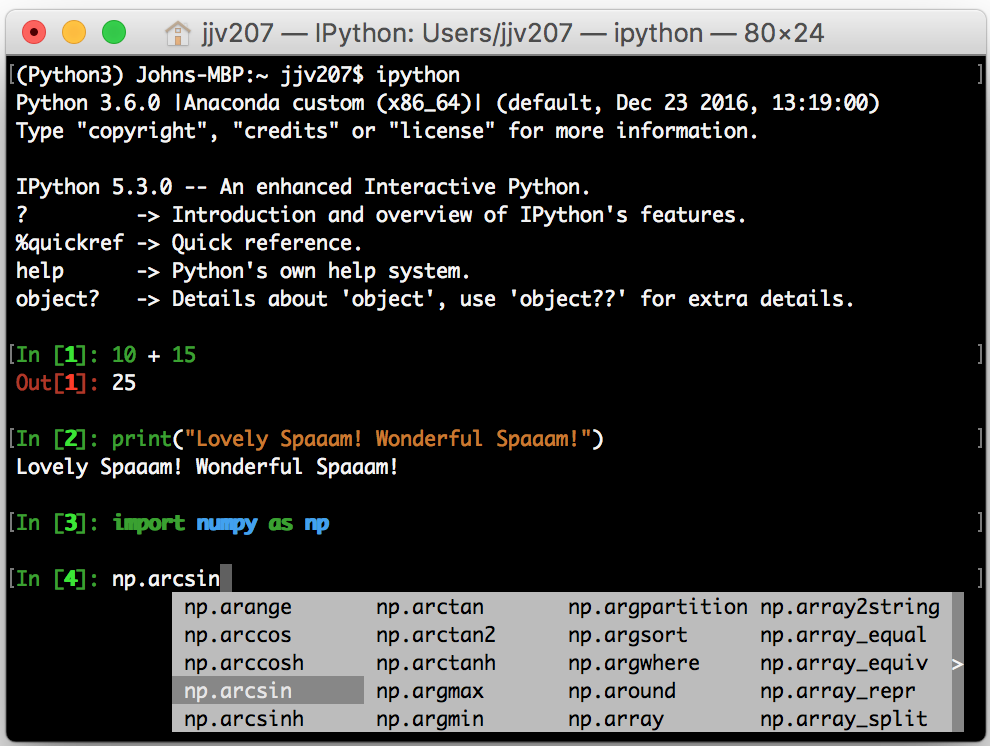
\includegraphics[width=0.6\textwidth]{ipython.png}
\end{center}
\end{frame}

%=============================================================================%
%=============================================================================%
\begin{frame}[fragile]
\frametitle{Executing Python code: Spyder IDE}
\begin{itemize}\addtolength{\itemsep}{.7\baselineskip}
	\item Spyder is an integrated development environment (IDE) for scientific computing, akin to \href{https://www.rstudio.com/}{RStudio} and \href{https://uk.mathworks.com/products/matlab.html}{MATLAB} 
	\item One place to write, execute and debug code, and explore variables
\end{itemize}

\begin{center}
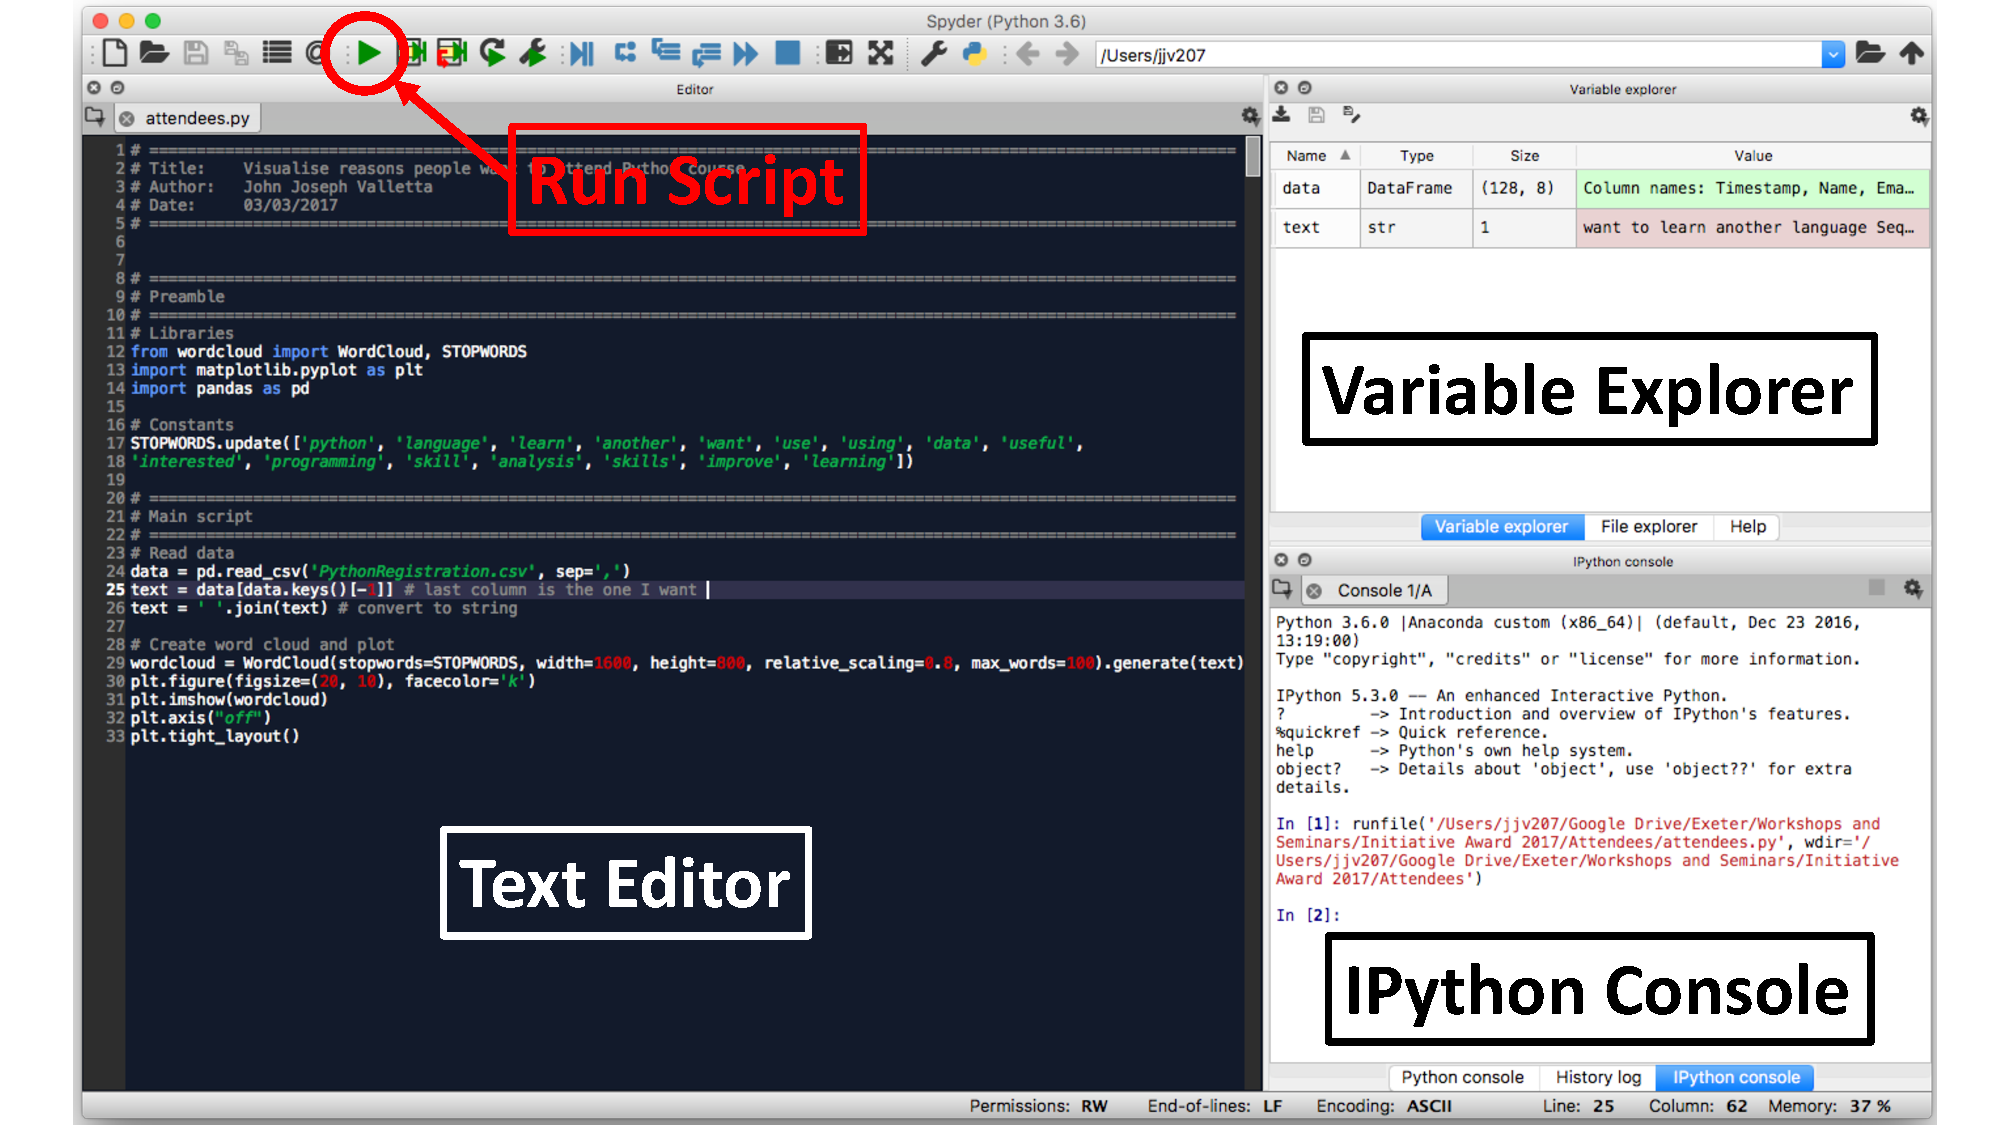
\includegraphics[width=0.8\textwidth]{spyder_annotated.pdf}
\end{center}
\end{frame}

%=============================================================================%
%=============================================================================%
% \begin{frame}[fragile]
% \frametitle{The Zen of Python}
% \begin{itemize}
% 	\item Coding standards are important in \textit{every} programming language%, but particular emphasis is placed in Python
% 	\item \href{https://www.python.org/dev/peps/pep-0008/}{PEP 8} is a style guide for python code  
% 	%\item If in doubt, be \textbf{consistent} in the way you structure your code
% \end{itemize}

% \scriptsize
% \begin{verbatim}
% Beautiful is better than ugly.
% Explicit is better than implicit.
% Simple is better than complex.
% Complex is better than complicated.
% Flat is better than nested.
% Sparse is better than dense.
% Readability counts.
% Special cases aren't special enough to break the rules.
% Although practicality beats purity.
% Errors should never pass silently.
% Unless explicitly silenced.
% In the face of ambiguity, refuse the temptation to guess.
% There should be one-- and preferably only one --obvious way to do it.
% Although that way may not be obvious at first unless you're Dutch.
% Now is better than never.
% Although never is often better than *right* now.
% If the implementation is hard to explain, it's a bad idea.
% If the implementation is easy to explain, it may be a good idea.
% Namespaces are one honking great idea -- let's do more of those!
% \end{verbatim}
% \normalsize
% \end{frame}

%=============================================================================%
%=============================================================================%
\begin{frame}{Python 2.x vs 3.x}
\centering
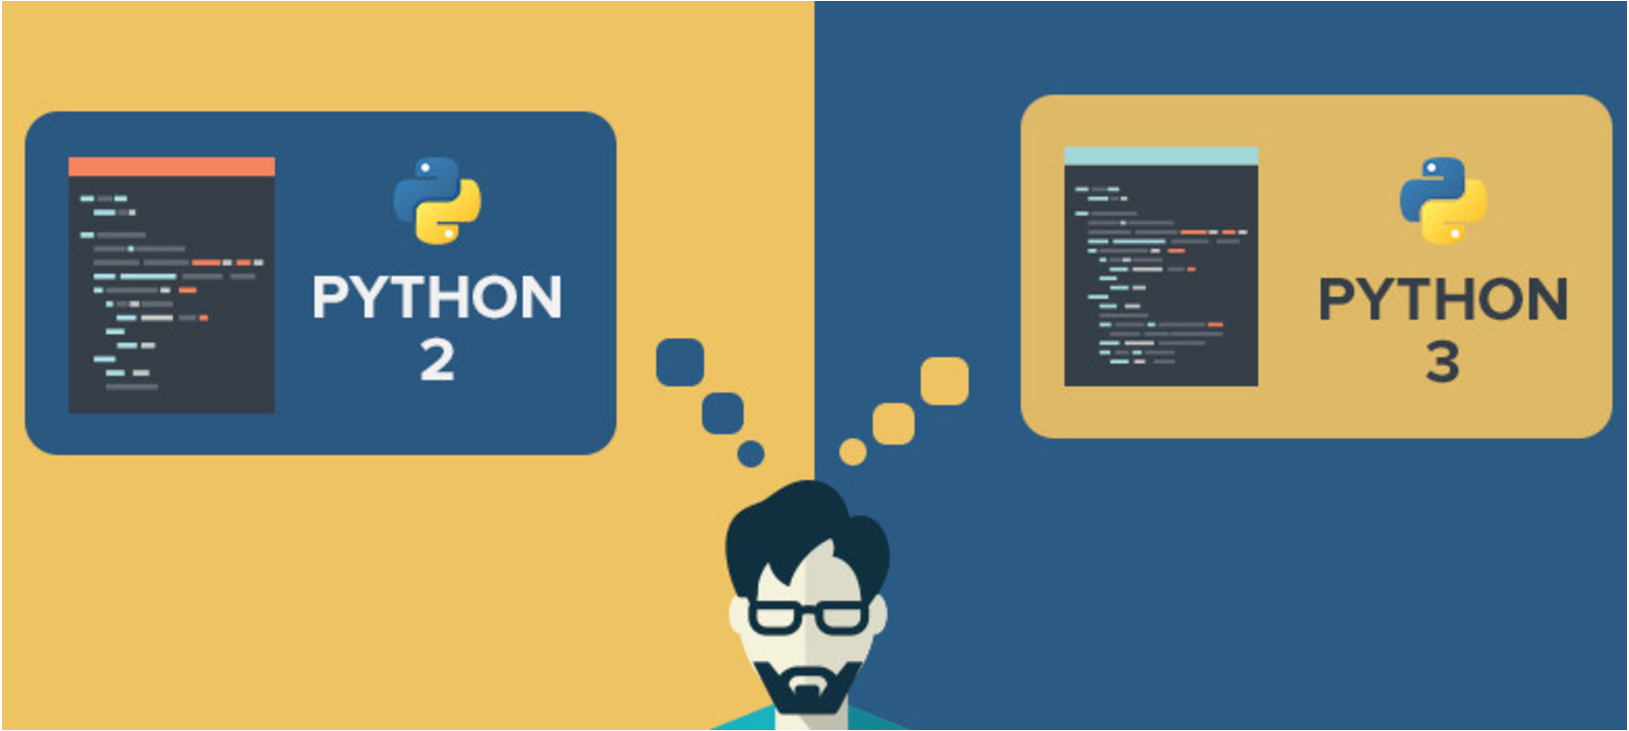
\includegraphics[width=.6\textwidth]{python2vs3.pdf}

\begin{itemize}\addtolength{\itemsep}{0.3\baselineskip}
	\item<1-> Python 2.x and Python 3.x are the two main versions of Python
	\item<2-> \href{https://wiki.python.org/moin/Python2orPython3}{Python 2.x is legacy, Python 3.x is the present and future of the language}
	\item<3-> However, not all Python 3.x code is backwards-compatible
	\item<4-> Be aware of \href{http://sebastianraschka.com/Articles/2014_python_2_3_key_diff.html}{key differences} between the two
	\item<5-> Here we will use Python 3.x, the language actively being developed
\end{itemize}
\end{frame}

%=============================================================================%
%=============================================================================%
\begin{frame}{Installing Python}
\begin{itemize}\addtolength{\itemsep}{0.5\baselineskip}
	\item The easiest way to get started is to download and install a cross-platform Python distribution such as:
	\begin{itemize}
		\item \href{https://www.continuum.io/downloads}{Anaconda}
		\item \href{https://store.enthought.com/downloads/}{Enthought Canopy}
	\end{itemize}
	\item These distributions contain several scientific libraries to get started
	\item Here we will use the Anaconda Python distribution and Spyder/IPython to write and run our code  
\end{itemize}

\begin{figure}

\includegraphics[width=.45\textwidth]{anaconda.png}\hfill
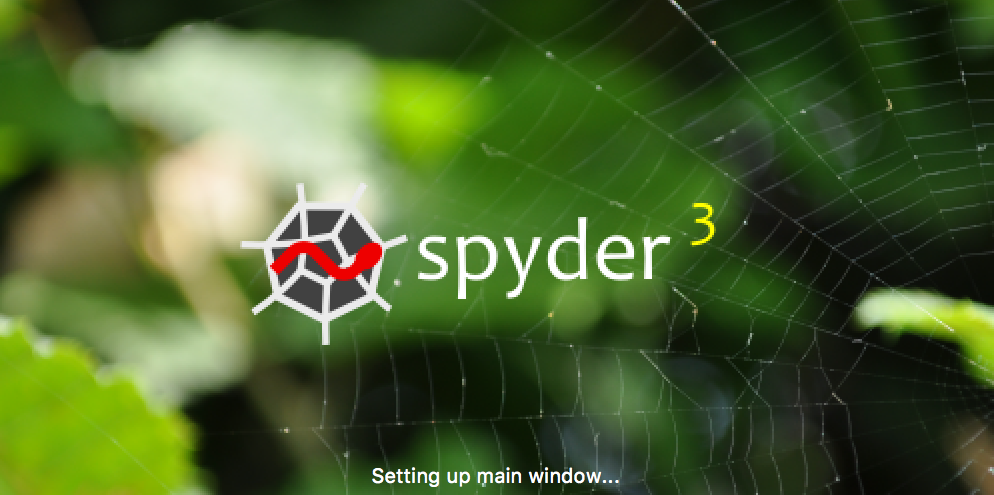
\includegraphics[width=.45\textwidth]{spyder.png}
\end{figure}

\end{frame}

%=============================================================================%
%=============================================================================%
% End of Document
%=============================================================================%
%=============================================================================%
\end{document}
